%Warning--I didn't find a database entry for "Hirschfeld2002"
%Warning--I didn't find a database entry for "Ceccato2008"
%Warning--I didn't find a database entry for "Tonella2005"
%Warning--I didn't find a database entry for "Binkley2005"
%Warning--I didn't find a database entry for "Deursen2005"
%Warning--I didn't find a database entry for "Hannemann2003"
%Warning--I didn't find a database entry for "Silva2009"
%Warning--I didn't find a database entry for "Rijst2008"
%Warning--I didn't find a database entry for "Marin2009"
%Warning--I didn't find a database entry for "Hannemann2005"
%Warning--I didn't find a database entry for "Bouchenak2006"
%Warning--I didn't find a database entry for "Loughran2004"


% % % % % % % % % % % % % % % % % % % % % % % % % % % % % % % % % %
%\documentclass[runningheads]{llncs}
\documentclass[preprint,10pt]{sigplanconf}

% packages
\usepackage{xspace}
\usepackage{ifthen}
\usepackage{amsbsy}
\usepackage{amssymb}
\usepackage{balance}
\usepackage{booktabs}
\usepackage{graphicx}
\usepackage{multirow}
\usepackage{needspace}
\usepackage{microtype}
\usepackage{bold-extra}
\usepackage{array}
\usepackage{epstopdf}


% references
\usepackage[colorlinks]{hyperref}
\usepackage[all]{hypcap}
\setcounter{tocdepth}{2}
\hypersetup{
	colorlinks=true,
	urlcolor=black,
	linkcolor=black,
	citecolor=black,
	plainpages=false,
	bookmarksopen=true}

\def\chapterautorefname{Chapter}
\def\appendixautorefname{Appendix}
\def\sectionautorefname{Section}
\def\subsectionautorefname{Section}
\def\figureautorefname{Figure}
\def\tableautorefname{Table}
\def\listingautorefname{Listing}

% source code
\usepackage{xcolor}
\usepackage{textcomp}
\usepackage{listings}
\definecolor{source}{gray}{0.9}
\lstset{
	language={},
	% characters
	tabsize=3,
	upquote=true,
	escapechar={!},
	keepspaces=true,
	breaklines=true,
	alsoletter={\#:},
	breakautoindent=true,
	columns=fullflexible,
	showstringspaces=false,
	basicstyle=\footnotesize\ttfamily,
	% background
	frame=single,
    framerule=0pt,
	backgroundcolor=\color{source},
	% numbering
	numbersep=5pt,
	numberstyle=\tiny,
	numberfirstline=true,
	% captioning
	captionpos=b,
	% formatting (html)
	moredelim=[is][\textbf]{<b>}{</b>},
	moredelim=[is][\textit]{<i>}{</i>},
	moredelim=[is][\color{red}\uwave]{<u>}{</u>},
	moredelim=[is][\color{red}\sout]{<del>}{</del>},
	moredelim=[is][\color{blue}\underline]{<ins>}{</ins>}}
\newcommand{\ct}{\lstinline[backgroundcolor=\color{white},basicstyle=\footnotesize\ttfamily]}
\newcommand{\lct}[1]{{\small\tt #1}}

% tikz
% \usepackage{tikz}
% \usetikzlibrary{matrix}
% \usetikzlibrary{arrows}
% \usetikzlibrary{external}
% \usetikzlibrary{positioning}
% \usetikzlibrary{shapes.multipart}
% 
% \tikzset{
% 	every picture/.style={semithick},
% 	every text node part/.style={align=center}}
% \tikzexternalize[prefix=figures/]{quality}

% proof-reading
\usepackage{xcolor}
\usepackage[normalem]{ulem}
\newcommand{\ra}{$\rightarrow$}
\newcommand{\ugh}[1]{\textcolor{red}{\uwave{#1}}} % please rephrase
\newcommand{\ins}[1]{\textcolor{blue}{\uline{#1}}} % please insert
\newcommand{\del}[1]{\textcolor{red}{\sout{#1}}} % please delete
\newcommand{\chg}[2]{\textcolor{red}{\sout{#1}}{\ra}\textcolor{blue}{\uline{#2}}} % please change
\newcommand{\chk}[1]{\textcolor{ForestGreen}{#1}} % changed, please check

% comments \nb{label}{color}{text}
\newboolean{showcomments}
\setboolean{showcomments}{true}
\ifthenelse{\boolean{showcomments}}
	{\newcommand{\nb}[3]{
		{\colorbox{#2}{\bfseries\sffamily\scriptsize\textcolor{white}{#1}}}
		{\textcolor{#2}{\sf\small$\blacktriangleright$\textit{#3}$\blacktriangleleft$}}}
	 \newcommand{\version}{\emph{\scriptsize$-$Id$-$}}}
	{\newcommand{\nb}[2]{}
	 \newcommand{\version}{}}
\newcommand{\rev}[2]{\nb{Reviewer #1}{red}{#2}}
\newcommand{\ab}[1]{\nb{Alexandre}{blue}{#1}}
\newcommand{\sv}[1]{\nb{Santiago}{orange}{#1}}
\newcommand{\ga}[1]{\nb{Gabriela}{blue}{#1}}

% graphics: \fig{position}{percentage-width}{filename}{caption}
\DeclareGraphicsExtensions{.png,.jpg,.pdf,.eps,.gif}
%\graphicspath{{figures/}}
\newcommand{\fig}[4]{
	\begin{figure}[#1]
		\centering
		\includegraphics[width=#2\textwidth]{#3}
		\caption{\label{fig:#3}#4}
	\end{figure}}
\newcommand{\largefig}[4]{
	\begin{figure*}[#1]
		\centering
		\includegraphics[width=#2\textwidth]{#3}
		\caption{\label{fig:#3}#4}
	\end{figure*}}

% abbreviations
\newcommand{\ie}{\emph{i.e.,}\xspace}
\newcommand{\eg}{\emph{e.g.,}\xspace}
\newcommand{\etc}{\emph{etc.}\xspace}
\newcommand{\etal}{\emph{et al.}\xspace}

% lists
\newenvironment{bullets}[0]
	{\begin{itemize}}
	{\end{itemize}}

\newcommand{\seclabel}[1]{\label{sec:#1}}
\newcommand{\secref}[1]{Section~\ref{sec:#1}\xspace}
\newcommand{\figlabel}[1]{\label{fig:#1}}
\newcommand{\figref}[1]{Figure~\ref{fig:#1}\xspace}

% D O C U M E N T
% % % % % % % % % % % % % % % % % % % % % % % % % % % % % % % % % %
\begin{document}

% T I T L E
% % % % % % % % % % % % % % % % % % % % % % % % % % % % % % % % % %

\title{Memoization Aspects: a Case Study}

\authorinfo{Santiago Vidal}
	{ISISTAN Research Institute, Faculty of Sciences, UNICEN University, Campus Universitario, Tandil, Buenos Aires, Argentina, Also CONICET}
	{svidal@exa.unicen.edu.ar}
\authorinfo{Claudia Marcos} 
	{ISISTAN Research Institute, Faculty of Sciences, UNICEN University, Campus Universitario, Tandil, Buenos Aires, Argentina, Also CIC}
	{cmarcos@exa.unicen.edu.ar}
\authorinfo{Alexandre Bergel}
	{PLEIAD Lab, Department of Computer Science (DCC), University of Chile, Santiago, Chile}
	{http://bergel.eu}
\authorinfo{Gabriela Ar\'evalo}
	{Universidad Nacional de Quilmes, Bernal, \\ Buenos Aires, Argentina, Also CONICET}


\maketitle

% A B S T R A C T
% % % % % % % % % % % % % % % % % % % % % % % % % % % % % % % % % %

\begin{abstract}
\chg{Unanticipated evolution of software is an activity difficult to realize. This paper presents a maintenance problem we faced while trying to evolve Mondrian, an open-source visualization engine: caches are now irrelevant with planned extension of Mondrian. The solution we adopted is to refactor these caches into a well defined aspect. This has been achieved without incurring a runtime penalty.} {During evolution phases of software, unanticipated changes are difficult to grasp. Mondrian, an open-source visualization engine, uses caching mechanism to store precalculated values avoiding calculating them when they are needed in the application. However, in the planned extensions of this tool, we have noticed that the caches are not relevant \ga{no me gusta esa palabra, pero no encuentro otra}. To solve this issue, we have refactored these caches into a well defined aspect. We have achieved it without incurring a runtime penalty \ga{qu\'e significa esta \'ultima frase}}

\end{abstract}

%: % % % % % % % % % % % % % % % % % % % % % % % % % % % % % % % % %
\section{Introduction}\seclabel{introduction}

%problem
\ga{Los primeros dos p\'arrafos no me convencen. Voy a reescribir o mejorar el texto}
Coping with emerging requirements is probably one of the most difficult challenges in software engineering~\cite{Somm00a}. 

This paper presents a solution to a maintenance problem we recently faced while developing the Mondrian application.
Mondrian is an agile visualization engine. It is used in more than a dozen projects. As in many software developments, new requirements set by the increasing set of clients have an impact on assumptions that were hold for years. 

Mondrian uses simple two-dimensions rendering to graphically visualize a target domain. Mondrian is almost exclusively used to visualize software metrics. It allows for a wide range of visual representations\footnote{\url{http://www.moosetechnology.org/docs/visualhall}}.
One of the strong assumptions that Mondrian holds is the structure of its multiple cache mechanisms. 

Mondrian has 9 caches spread over the graphical element hierarchy. 
The caches aim to quickly render two dimensional widgets, graphically composed of rectangle and line shapes. Mondrian caches are instances of the memoization technique\footnote{\url{http://www.tfeb.org/lisp/hax.html\#MEMOIZE}}. Sending twice the same message returns the same value if there is no side effect that impacts the computation. 

Unfortunately, the new requirements of Mondrian defeats the purpose of some of the caches it defines. One example is the bounds computation to obtain the circumscribed rectangle of a two-dimensional graphical element. This cache is senseless in a 3D setting. Bypassing the cache results in a complex extension of Mondrian.

%solution
We have first identified where the caches are implemented and how they interact with the rest of the application.
For each cache, we marked methods that initialize the cache and reset it. 
We have subsequently undertaken a major refactoring of Mondrian's core: we have produced a prototyping version of Mondrian in which caches are externalized from the base code. Our refactoring was implemented with a custom aspect mechanism \ga{qu\'e es esto? qu\'e es un custom?}.

%surprising result
We were able to modularize the cache while preserving the overall architecture and Mondrian performances did not suffer from the refactoring.

%contribution
The contributions of this paper are: (i) identification of memoizing cross-cutting concern and (ii) refactorization of these cross-cutting concerns into modular and pluggable aspects.
%\item lesson learnt

%outline
The paper is structured as follows.
\secref{problem} shows the problem we faced with when trying to evolve Mondrian.
\secref{refactoring} describes the aspect-based solution we adopted.
\secref{results} presents the impacts of our solution on Mondrian.
\secref{relatedWork} briefly summarizes the related work.
\secref{conclusion} presents some conclusions.


%The story to tell in this paper is the following one:
%1) We have the actual Mondrian code
%2) Santiago have extracted the CC into annotations
%3) He has identified different possible pragmas. Here some patterns could be identified based on the code (That's the POINT of the paper)
%4) Once we have the pragmas, we can think of an injection machine to produce new code.
%This new code is semantically equivalent to the original one, but not syntactically the same. This is not so important since all the large set of Mondrian unit tests has the last word on it.
%
%Then the core of the paper will be the Different patterns of hand written code that are rewritten (refactored?) with pragmas 
%
%justificar el xq se quiere refactorizar los cache 
%
%\ab{what is the link with your previous work? Is there some hypothesis that you validate with the experiment on Mondrian?}
%
%\ab{this is just a try, we will probably refine that later} This work presented in this paper makes the following contributions:
%\begin{itemize}
%\item Identification and composition of pattern for memoization techniques
%\item Associating code quality metrics and AOP-based refactoring. \ab{refactoring Mondrian increases its quality (we can use macCabe complexity, number of lines of code, number of methods, ...)}
%\item General technique of implementing memoization with AOP
%\end{itemize}

%: % % % % % % % % % % % % % % % % % % % % % % % % % % % % % % % % %
\section{Making Mondrian Evolve}\seclabel{problem}

This section details a maintenance problem we have faced with when developing Mondrian.

%=========
\subsection{Turning Mondrian into a framework}

Mondrian\footnote{\url{http://www.moosetechnology.org/tools/mondrian}} is an agile visualization library ~\cite{Meye06a}. A domain specific language is provided to easily define interactive visualizations.
Visualizations are structured along a graph structure, made of nested nodes and edges. Mondrian is a crucial component, used in more than a dozen independent projects. To meet clients performance requirements, Mondrian authors are paying a great attention to provide fast and scalable rendering. To that purpose, Mondrian contains a number of caches to avoid redundant code executions.

Mondrian is on the way to become a visualization engine framework more than a library as it is currently. Mondrian is now used in situations that were not originally planned. For example, Mondrian has been used to visualize the real-time behavior of animated robots\footnote{\url{http://www.squeaksource.com/Calder.html}}, 3D visualizations\footnote{\url{http://www.squeaksource.com/Klotz.html}}, whereas Mondrian has been originally designed to visualize software source code using plain 2D drawing~\cite{Lanz03d}. The caches that are intensively used when visualizing software are not useful and may even be a source of slowdown and complexity when visualizing animated robots. 

%The future Mondrian framework must offer the possibility of selectively using and combining caches.

%=========
\subsection{Memoization}

Memoization is an optimization technique used to speed up an application by making calls avoid repeating the similar previous computation. Consider the method \texttt{absoluteBounds} that any Mondrian element can answer to. This method determines the circumscribed rectangle of the graphical element:

\begin{lstlisting} 
MOGraphElement>>absoluteBounds
	<b>absoluteBoundsCache 
		ifNotNil: [ ^ absoluteBoundsCache ].</b>
	^ <b>absoluteBoundsCache := 
		</b>self shape absoluteBoundsFor: self
\end{lstlisting}

The method \ct{absoluteBoundsFor:} implements a heavy computation to determine the smallest rectangle that contains all the nested elements. Since this method does not perform any global side effect, the class \ct{MOGraphElement} defines an instance variable called \ct{absoluteBoundsCache} which is initialized at the first invocation of \ct{absoluteBounds}. Subsequent invocation will therefore use the result previously computed. 

Obviously, the variable \ct{absoluteBoundsCache} needs to be set to \ct{nil} when the bounds of the element are modified (\eg adding a new nested node, drag and dropping).

%Implementing a memoization is not always that simple. 

%=========
\subsection{Problem}

Mondrian intensively uses memoization for most of its computation. A user-performed interaction that leads to an update of the visualization invalidates the visualization. These memoization were gradually introduced over the development of Mondrian (which started in 2006). Each unpredicted usage \ga{qu\'e es unpredicted usage? una extensi\'on?} leaded to a performance problem that has been solved using a new memoization. There are about 32 memoizations in the current version of Mondrian.

These caches have been shaped along the common usage of Mondrian. Visualizations produced in Mondrian are \emph{all} static, employ colored geometrical objects.

Extending the range of applications for Mondrian turns some of the caches senseless. For example \ct{absoluteBoundsCache} has no meaning in the three-dimensional version of Mondrian since the circumscribed rectangle is meaningful only with two dimensions.

\paragraph{Using delegation.}
We first tried to address this problem by relying only on explicit objects, one for each cache. This object would offer the needed operations for accessing and resetting a cache.

As exemplified with the \ct{absoluteBounds} method given above, the caches are implemented by means of dedicated instance variables defined in the \ct{Cache} class. That is to say, each cache is associated with an instance variable. In this way, a variable of the Cache class, called \ct{generalCache}, is defined in the \ct{MOGraphElement} class. Through this variable the different caches can be accesed by mean of the \ct{cacheAt:(key)} method where \ct{key} is a string with the name of the cache.
%The goal of the refactoring is the extraction of the \emph{Cache Concern} by means of the creation of a specific class to delegate the behavior of the caches\ab{Do we need this sentence, I guess no}. 

%To accomplish this task could be used, for example, a strategy which uses a class containing a collection of caches and each cache can contain different types of items (as is shown in Fig. \ref{fig:Cache-behaviour-delegation.}). 
\figref{Cache-behaviour-delegation} illustrates this situation where a graph element has one instance of the \ct{Cache} class, itself referencing to many instances of \ct{CacheableItem}, one for each cache.
%In this case, all the cache variables and the fragments of code of the methods in which they were used were encapsulated using the \emph{Cache} class and creating a suitable \emph{CacheableItem}. So, with this solution, only remain a reference in \emph{MOGraphElement} class to the \emph{Cache} class that contains all the caches\ab{I do not understand. Did I just say that?} \sv{trato de justificar que se gana con esta solucion. Lo bueno era que solo quedaba una referencia a la clase contenedora de los caches en MOGraphElement}. 

Below we show how the \ct{absoluteBounds} method is written following this approach:  
\begin{lstlisting} 
MOGraphElement>>absoluteBounds
	<b>(generalCache cacheAt: 'absoluteBoundsCache')</b> ifCacheNil: [
	<b>(generalCache cacheAt: 'absoluteBoundsCache')</b>
	 putElement: (self shape absoluteBoundsFor: self)].
	^ <b>(generalCache cacheAt: 'absoluteBoundsCache')</b> getInternalCache.
\end{lstlisting}
As can be seen, with this approach the different instance variables related with the caches are replaced by a unique variable called \ct{generalCache}. On the other hand, the legibility of the method is deteriorated as well as the performance.

\paragraph{Significant overhead.} This modularization solely based on delegating message has a significant overhead at execution time
because of additional indirection.
The separation of this concern is not a trivial problem. \ga{la siguiente frase no la entiendo} Specifically,
when we use this solution, the caches mechanism was 3 to 10 times slower,
being the delay proportional to the number of elements.

%
\begin{figure*}
\begin{centering}
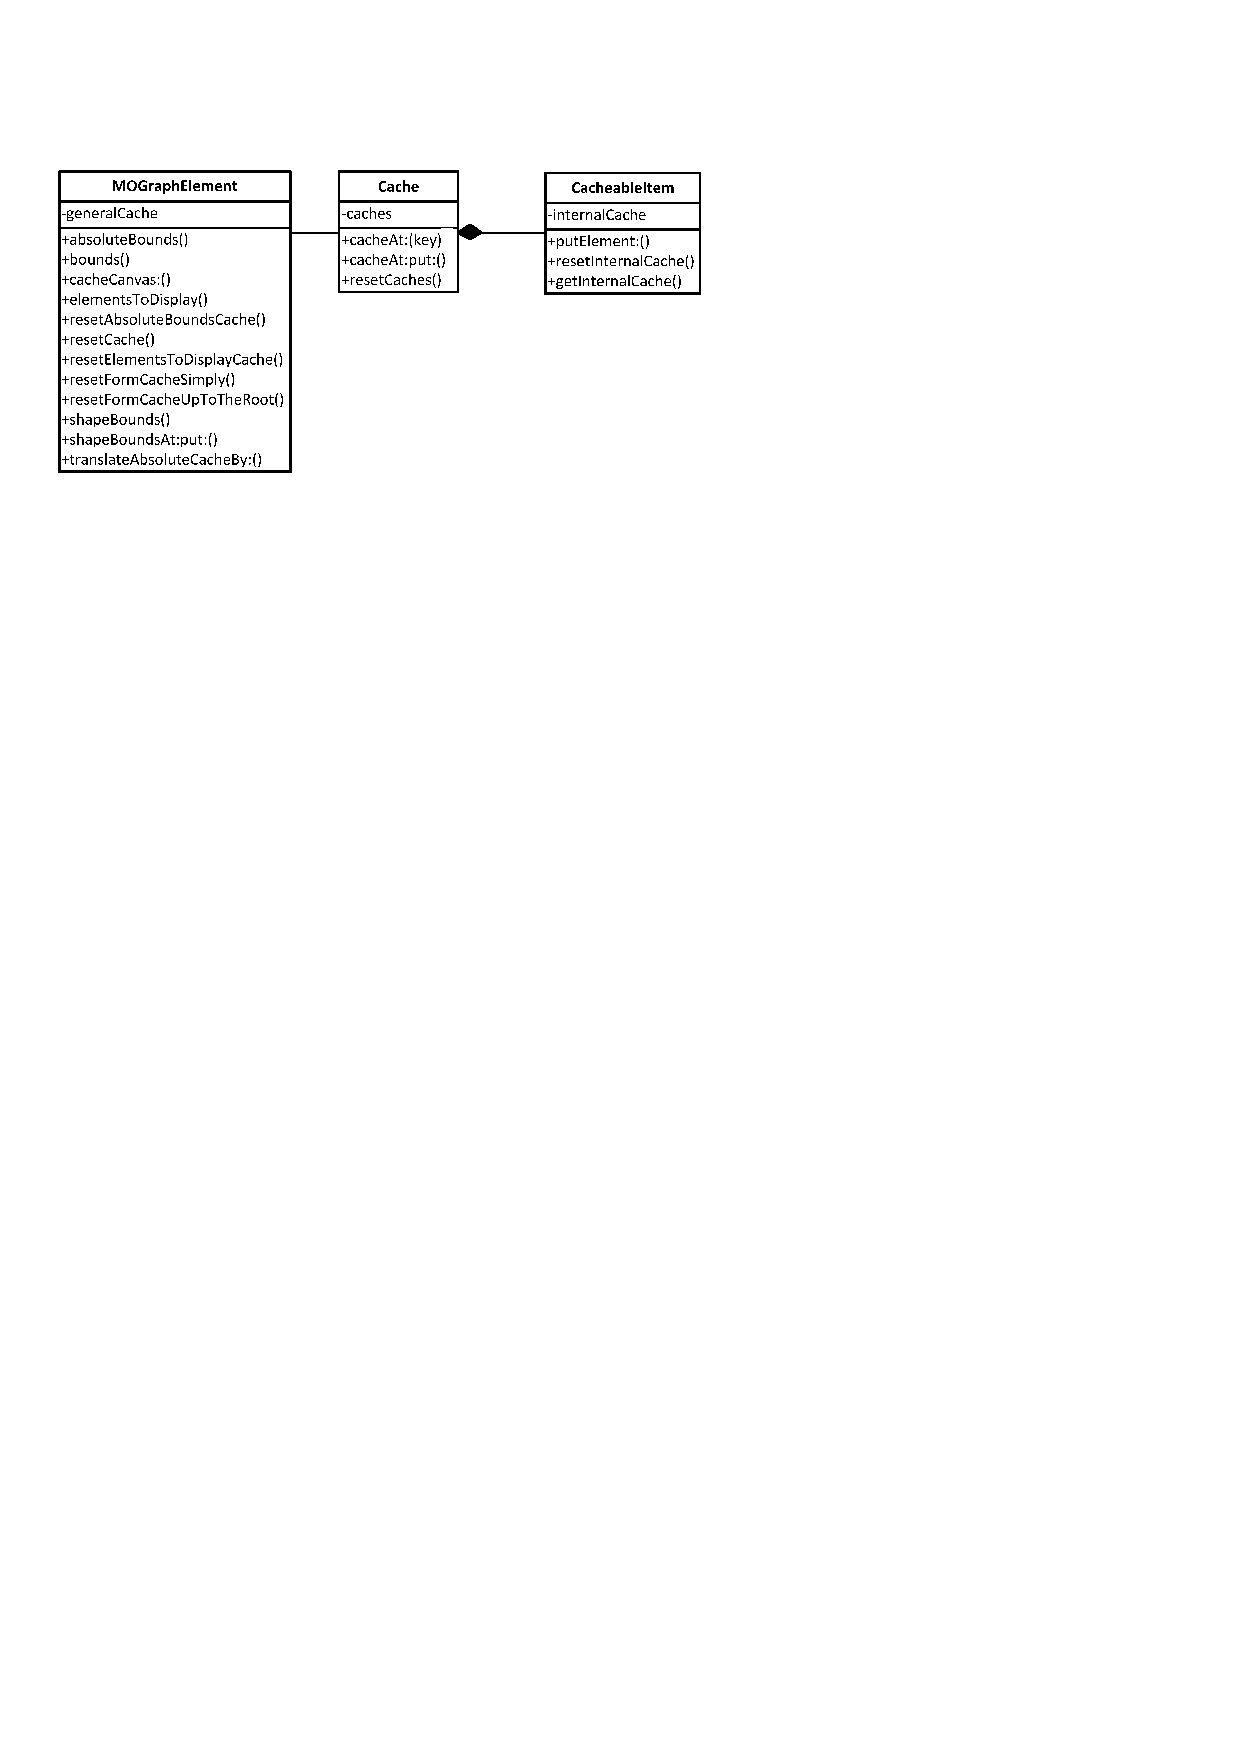
\includegraphics[bb=27bp 615bp 338bp 762bp,scale=0.97]{CacheMechanisms} 
\par\end{centering}

\caption{Cache behavior delegation.\label{fig:Cache-behaviour-delegation}}

\end{figure*}


%=========
\subsection{Requirement for refactoring}

\ga{La siguiente frase la tengo que reescribir} Refactoring Mondrian is a task that has to be performed carefully. In particular, the refactoring has to follow the constraints:

\begin{itemize}
\item All cache accesses have to be identified. This is essential to have all the caches equally considered. 
\item No cost of performance must be incurred, else it defeats the whole purpose of the work.
\item Readability must not be reduced.
\end{itemize}

%: % % % % % % % % % % % % % % % % % % % % % % % % % % % % % % % % %
\section{Aspect-based Refactoring}\seclabel{refactoring}


The goal of the refactoring is the separation of the \emph{Cache
Concern} from the four essential classes of \emph{Mondrian}: \emph{MOGraphElement}
and its subclasses (\emph{MOEdge}, \emph{MONode}, and \emph{MORoot}). These classes total 235 methods and more than 1000 number of lines of codes.

%========
\subsection{Identifying caches}
The first step of the refactoring is identifying the caches.
This initial identification of the caches is done with the information
provided by the developers of Mondrian and is based on knowing the
variables related to the caches and the places where they are used. The caches are mostly identified by browsing the methods in which the caches variables are referenced and accessed.
Nine different caches are found in Mondrian: \emph{cacheShapeBounds},
\emph{cacheForm}, \emph{boundsCache}, \emph{absoluteBoundsCache},
\emph{elementsToDisplayCache}, \emph{lookupNodeCache}, \emph{cacheFromPoint},
\emph{cacheToPoint}, and \emph{cacheBounds}. Each of them has a different
internal structure according to what is stored: \emph{boundsCache} will hold an instance of the class \ct{Rectangle} and \emph{cacheForm} an instance of a bitmap \ct{Forms}, for example.


After this initial identification, the fragment of codes in which the caches are used
are grouped together based on the purpose of its use (\eg saving information, obtaining the data stored). Each group is associated with different activities:
\begin{itemize}
\item Initialize and reset the cache: the fragments of code in this group initialize or reset a cache variable putting them in nil or creating an instance of an object.
\item Retrieve the cache value: this group obtains the information that is saved in a cache.
\item Store data in the cache: the code fragments grouped here store information into a cache variable.
\end{itemize}
%The task of group the fragments of code of the different caches is
%achieved with the goal of identifying possible strategies for refactoring\ab{I do not understand this sentence. ``The task of group'' ?}\sv{Mas arriba habia puesto "the fragment of codes in which the caches are used
%are grouped together based on the purpose of its use". A eso me refiero con "The task of group", la tarea de agrupar el codigo segun lo que hacen}.

These groups allow the identification of code patterns that are
repeated in the use of the caches. For each found pattern an aspect refactoring is associated ~\cite{Kellens2007}. These code patterns are described in the following subsections.

%========
\subsection{Pattern description}\seclabel{Pattern-Identification}


We identified 5 code patterns based on Mondrian source code and are described below.
Each pattern is described with a relevant typical occurrence,
the number of occurrences we found in Mondrian and an illustration.

\paragraph{Reset Cache.} A cache has to be invalidated when its content has to be updated. We refer to this action as reset. The code to express a reset is \emph{cache:=resetValue} where
\emph{resetValue} and the initial value the cache has to have \sv{Is something missing here?}. Typically, the \emph{resetValue} depends on the type of the stored value. It could be \ct{nil}, an empty dictionary, or a particular value (\eg \ct{0@0}).
Eighteen occurrences of this pattern are found in Mondrian. 
We found that in some occurrences the reset of the caches is performed before the logic of the method, and other methods in which the reset must be done after. For example, the method \ct{MOGraphElement>>shapeBoundsAt:put:} resets the caches \emph{absoluteBoundsCache} and \emph{boundsCache} before modifying the cache cacheShapeBounds. In contrast, the method \ct{MONode>>translateBy:bounded:} resets the caches \emph{boundsCache} and \emph{absoluteBoundsCache} after executing most of the sentences of the method. 

Consider the method \ct{MOGraphElement>>resetCache}. This method is called whenever the user drags and drops a graphical element. In
this method the \emph{Reset Cache} pattern is repeated in four \ga{ puedo reemplazar "occasions" with "places"?}
to reset the caches \emph{boundsCache}, \emph{absoluteBoundsCache},
\emph{cacheShapeBounds}, and \emph{elementsToDisplayCache}. In this case, the reset of the caches can be done before or after the execution of the methods \emph{resetElementsToLookup} and  \emph{resetMetricCaches}.

\begin{lstlisting} 
MOGraphElement>>resetCache 
	self resetElementsToLookup.
	boundsCache := nil. 
	absoluteBoundsCache := nil. 
	cacheShapeBounds :=SmallDictionary new. 
	elementsToDisplayCache := nil. 
	self resetMetricCaches
\end{lstlisting}



\paragraph{Lazy Initialization.} In some situations it is not relevant to initialize the cache before it is actually needed. This happens when a graphical element is not outside the displayed window \ga{"is not outside" es "is inside"}: no cache initialization is required for a graphical element if the element is not displayed. These caches are relevant only when the user actually sees the element by scrolling the visualization. Typically, the structure of this pattern is: \emph{\^{} cache ifNil:[cache:=newValue]}. Mondrian contains five occurrences of a lazy cache initialization. Consider the \ct{bounds} method:

\begin{lstlisting} 
MOEdge>>bounds  
	^ boundsCache ifNil:[boundsCache:= self shape computeBoundsFor: self ]. 
\end{lstlisting}

The circumscribed rectangle is returned by \ct{computeBoundsFor:} and is performed only when an edge is actually visible (\ct{bounds} is used in \ct{drawOn:}, the rendering method).

\paragraph{Cache Initialization.} This pattern represents a situation in
which a value is assigned to a cache. The structure of the pattern
is only an assignation: \emph{cache := aValue}. This pattern is found
in three occasions. Consider the method \ct{cacheCanvas:}

\begin{lstlisting} 
MOGraphElement>>cacheCanvas: aCanvas 
	cacheForm:= aCanvas form 
	  copy: ((self bounds origin + aCanvas origin-(1@1)) 
				extent: (self bounds extent + (2@2))). 
\end{lstlisting}

The method \ct{cacheCanvas:} is invoked only during testing in order to verify some characteristics of the caches such as their effectiveness.

\paragraph{Return Cache.} This pattern shows the situation in which a cache
is accessed. The structure of the pattern is the return of the cache:
\emph{return cache}. This pattern is found in four occasions. Next, the method \ct{shapeBounds} is presented as an example in which
\emph{cacheShapeBounds} is accessed.

\begin{lstlisting} 
MOGraphElement>>shapeBounds  
	^ cacheShapeBounds
\end{lstlisting}

\paragraph{Cache Loaded.} This pattern checks whether one cache or more
are initialized or conversely, if they are not nil. So, the structure of the
pattern for a single cache is \emph{cache != nil}. This pattern is
found in two occasions. Next the method \emph{isCacheLoaded} is presented
as an example of this pattern.

\begin{lstlisting} 
MOGraphElement>>isCacheLoaded 
	^cacheForm notNil. 
\end{lstlisting}


Additionally, Table \ref{tab:Cache-Concern-scattering} gives the occurrences of each pattern in the \ct{MOGraphElement} hierarchy,
the methods involved in each pattern, and the caches related with
a pattern.

%
\begin{table*}
\begin{centering}
\begin{tabular}{|p{2.5cm}|c|c|p{3.5cm}|}
\hline 
Cache  & Occurrences  & Methods involved  & Caches involved\tabularnewline
\hline
\hline 
\emph{Reset Cache}  & 18 & 10 & boundsCache, absoluteBoundsCache, cacheShapeBounds, elementsToDisplayCache,
cacheForm, cacheFromPoint, cacheToPoint\tabularnewline
\hline 
\emph{Lazy Initialization}  & 5 & 5 & elementsToDisplayCache, absoluteBoundsCache, boundsCache, cacheBounds\tabularnewline
\hline 
\emph{Cache Initialization}  & 3 & 3 & cacheForm, cacheFromPoint, cacheToPoint\tabularnewline
\hline 
\emph{Return Cache}  & 4 & 4 & cacheShapeBounds, cacheForm, cacheFromPoint, cacheToPoint\tabularnewline
\hline 
\emph{Cache Loaded} & 2 & 2 & cacheForm, cacheFromPoint, cacheToPoint\tabularnewline
\hline 
Total  & 32 & 24 & \multicolumn{1}{c}{}\tabularnewline
\cline{1-3} 
\end{tabular}
\par\end{centering}

\caption{Cache Concern scattering summary.\label{tab:Cache-Concern-scattering}}

\end{table*}

\largefig{}{0.6}{PatternLocation}{Pattern locations in the MOGraphElement hierarchy}

%\begin{figure*}
%\begin{centering}
%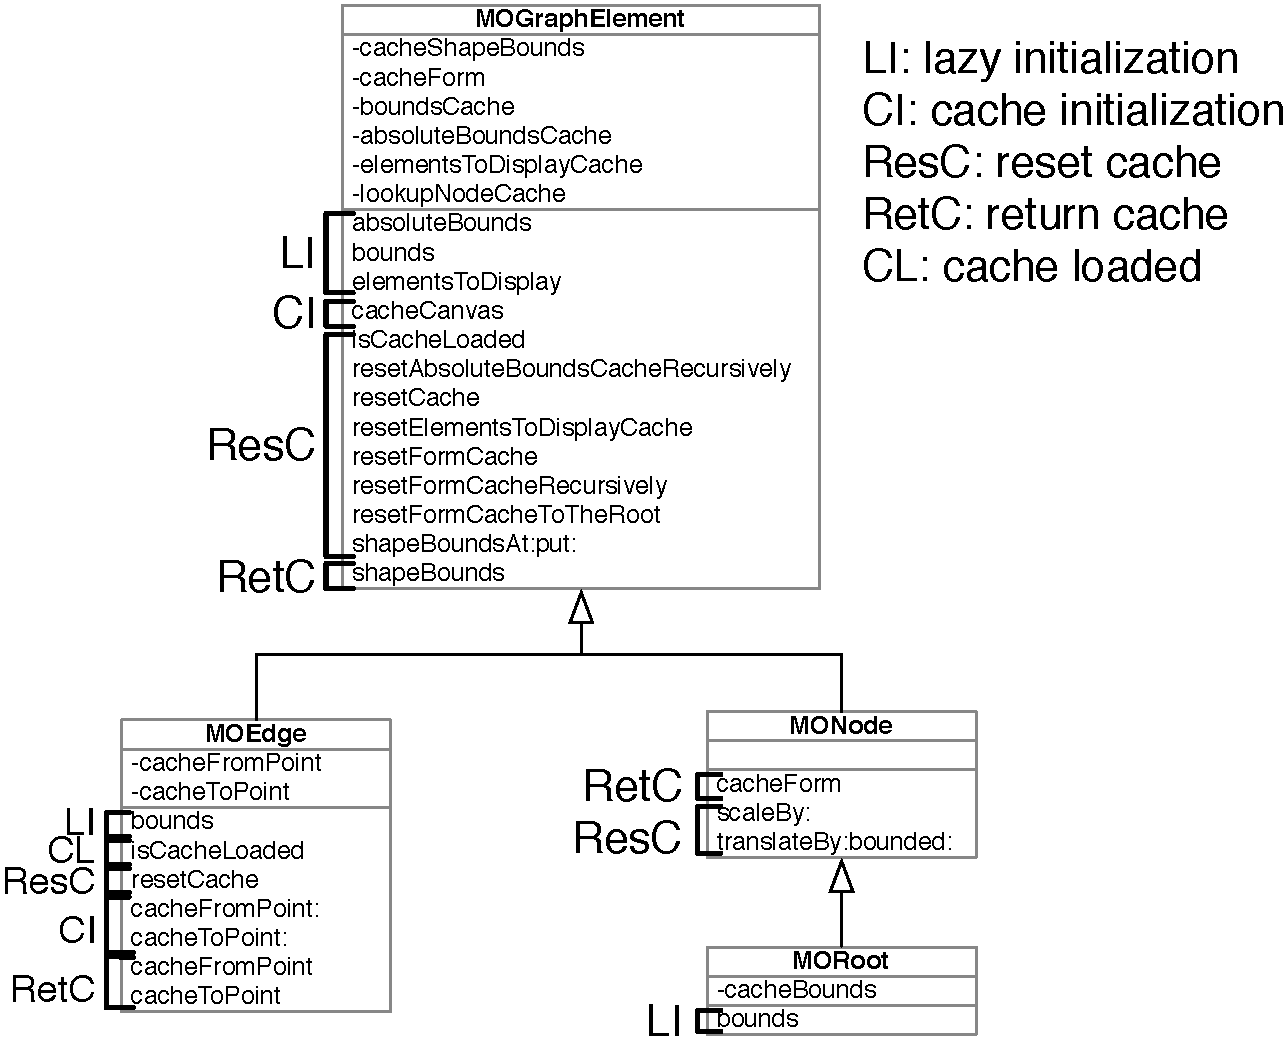
\includegraphics[bb=186bp 306bp 497bp 644bp,scale=0.9]{PatternLocation.pdf} 
%\par\end{centering}
%\caption{Pattern locations in MOGraphElement hierarchy.\label{fig:Pattern-locations-in}}
%\end{figure*}

\figref{PatternLocation} shows the distribution of the caches over the main Mondrian classes, methods in which the caches are used, and the classes where each cache is defined. As we can observe, the caches are used and defined across the whole class hierarchy.

%========
\subsection{Cache concerns as aspects}

Once the code patterns are identified, we set up strategies to refactor them. The goal of the refactorization is the separation of these patterns from the main code without changing the overall behavior, enforced by an extended set of unit tests.

The refactoring is performed by encapsulating each of the nine caches into an aspect. Aspect definition weaving is achieved via a custom AOP mechanism based on code annotation and source code manipulation.

%Several alternatives were explored to encapsulate the \emph{Cache
%Concern}. After exploring a variety of options such as the separation
%of the concern by means of the definition of an exclusive class for
%managing caches or the use of proxies to
%intercept messages, an approach based on code injection was chosen.
%This solution has the advantage of encapsulating the concern in a
%new unit while the code that it is finally executed after the injection
%is similar to the original code of \emph{Mondrian}. So, the performance
%is not affected. In order to encapsulate the source code related with
%the code patterns the \emph{pragma} mechanism is used. \emph{Pragmas}
%are the method annotation syntax implemented by Pharo.

The refactoring strategy used is: for each method that involves a cache, the part of the method that directly deals with the cache is removed and the method is annotated.
%The decision to define the pragma inside the method is in order to allow a better visibility of the code that is injected. 
The annotation is defined along the cache pattern associated to the cache access removed from the method.
The annotations structure is \emph{$<$patternCodeName: cacheName$>$} where \emph{cacheName} indicates the name of the cache to consider and \emph{patternCodeName} indicates the pattern code to be generated. For example, the annotation \emph{$<$LazyInitializationPattern: \#absoluteBoundsCache$>$} indicates that the \emph{Lazy Initialization} pattern will be ``weaved'' for the cache \emph{absoluteBoundsCache} in the method in which the annotation is defined.

The weaving is done via a custom code injection mechanism \ga{otra vez el custom}. For each annotation a method may have, the code injector performs the needed source code transformation to use the cache. Specifically, the weaving is achieved through the following steps:

\begin{enumerate}
\item A new method is created with the same name that the method that contains
the annotation but with the prefix {}``compute'' plus the name of the
class in which is defined. For example, given the next method
\begin{lstlisting} 
MOGraphElement>>absoluteBounds
	<LazyInitializationPattern: #absoluteBoundsCache> 
	^ self shape absoluteBoundsFor: self
\end{lstlisting}
a new method called \ct{computeMOGraphElementAbsoluteBounds} is created.
\item The code of the original method is copied into the new method.
\begin{lstlisting} 
MOGraphElement>>computeMOGraphElementAbsoluteBounds
	^ self shape absoluteBoundsFor: self
\end{lstlisting}
\item The code inside the original method is replaced by the code automatically
generated according to the pattern defined in the annotation. This generated
method contains a call to the new method of the Step 1.
\begin{lstlisting} 
MOGraphElement>>absoluteBounds
	absoluteBoundsCache 
		ifNotNil: [ ^ absoluteBoundsCache].
	^ absoluteBoundsCache:=
		(self computeMOGraphElementAbsoluteBounds)
\end{lstlisting}
\end{enumerate}

In order to automatically generate the code to be injected, the code weaver uses a class hierarchy (\figref{Pattern-hierarchy}), rooted in the abstract \ct{CachePattern}.
\ct{CachePattern} contains the methods necessary for processing annotations (called pragmas in the Pharo terminology \ga{nunca se dijo previamente que Mondrian se basaba en Pharo}). Each subclass overrides \ct{generateMethodWith:} to perform the source code manipulation.

%Each cache pattern has to implements this interface which allow the
%generation of the methods mentioned above. Basically each subclass
%is responsible of the definition of the pragma to be used and the
%generation of the code sentences to be injected related with the cache
%whereas the interface \emph{CachePattern} creates the methods to be
%added to the system. This class hierarchy is shown in Fig. \ref{fig:Pattern-hierarchy.}.
%
\begin{figure*}
\begin{centering}
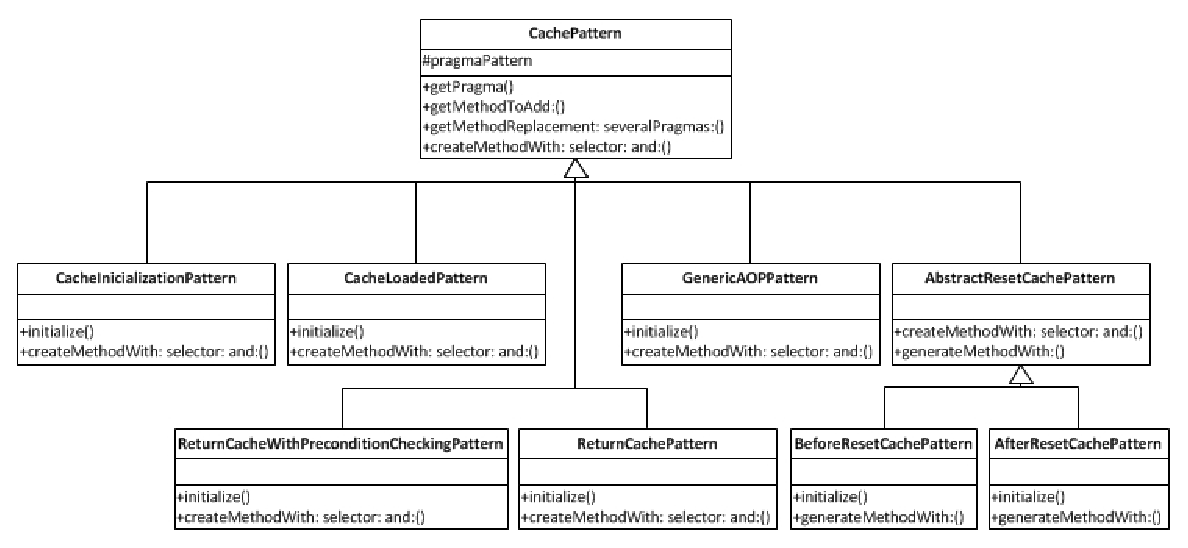
\includegraphics[bb=21bp 541bp 561bp 789bp,scale=0.7]{PatternInheritance}
\par\end{centering}

\caption{Pattern hierarchy.\figlabel{Pattern-hierarchy}}

\end{figure*}


Next, the refactorings applied to each code pattern are presented.

\paragraph{Reset Cache.} In order to refactor this pattern each statement
that resets a cache was extracted using an annotation. The annotation contains
the cache to be resetted. Since in some cases the resets are done
at the beginning of a method and others at the end, a hierarchy of
Reset Cache pattern is created. As shown in \figref{Pattern-hierarchy},
this hierarchy is composed of the classes \emph{AbstractResetCachePattern},
\emph{BeforeResetCachePattern}, and \emph{AfterResetCachePattern}.
The annotations are defined in the classes at the bottom of the hierarchy
as $<$BeforeResetCachePattern: cacheName$>$ and $<$AfterResetCachePattern:
cacheName$>$ respectively. For example, in the case presented in 
\secref{Pattern-Identification} of the method \emph{resetCache},
an annotation is defined for each reset of a cache leaving a cleaner code
in the method. In this case, all the resets are done before the method
call, so the used annotations are the ones defined by \emph{BeforeResetCachePattern}.
Even though the order of calls is changed (in comparison with the
original method), the method behavior is not modified. The code to
be generated will reset the cache defined
in the annotation. Following, the refactored code is presented:

\begin{lstlisting} 
MOGraphElement>>resetCache 
	<BeforeResetCachePattern: #absoluteBoundsCache> 
	<BeforeResetCachePattern: #elementsToDisplayCache>
	<BeforeResetCachePattern: #boundsCache> 
	<BeforeResetCachePattern: #cacheShapeBounds> 
	self resetElementsToLookup. 
	self resetMetricCaches
\end{lstlisting}

The methods \emph{resetElementsToLookup} and \emph{resetMetricCaches} perform additional actions that do not involve the cache variables. For this reason they remain in the \emph{resetCache} method.

After the code injection, the resetCache method is transformed into:

\begin{lstlisting} 
MOGraphElement>>resetCache 
	absoluteBoundsCache:=nil.
	elementsToDisplayCache:=nil. 
	boundsCache:=nil. 
	cacheShapeBounds:=SmallDictionary new. 
	self computeMOGraphElementresetCache 
\end{lstlisting}

where the method \ct{computeMOGraphElementresetCache} is:

\begin{lstlisting} 
MOGraphElement>>computeMOGraphElementresetCache
	self resetElementsToLookup. 
	self resetMetricCaches 
\end{lstlisting}

This mechanism of injection of the generated code is the same for
the rest of the patterns.

\paragraph{Lazy Initialization.} To refactor this pattern
the precondition checking is contained into an annotation defined as
$<$LazyInitializationPattern: cacheName$>$. Given that
the cache is initialized with a value when the precondition fails,
the original method is modified to return this value. For example,
in the case of the method \emph{bounds} introduced in the previous
section, the code related to the cache is extracted using the annotation
and only the value to initialize the cache remains in the method as
shown the code below:

\begin{lstlisting} 
MOEdge>>bounds 
	<LazyInitializationPattern: #boundsCache> 
	self shape computeBoundsFor: self. 
\end{lstlisting}

In this way, the code to be generated for this example will be \emph{boundsCache
ifNotNil: {[} \textasciicircum{} boundsCache{]}. \textasciicircum{}
boundsCache:= computeMOEdgeBounds.}

\paragraph{Cache Initialization.} The refactorization of this cache is
similar to the last one. Given that the structure of the pattern is
an assignment, the first section of the assignment (\emph{cacheName:=})
will be generated automatically by the weaver using an annotation $<$CacheInitializationPattern: cacheName$>$.
The value at which the cache is initialized constitutes the method body.
In the case of the example presented in \secref{Pattern-Identification},
the refactored code is shown below:

\begin{lstlisting} 
MOGraphElement>>cacheCanvas: aCanvas 
	<CacheInitializationPattern: #cacheForm>  
	(aCanvas form copy: ((self bounds origin + aCanvas origin
	- (1@1)) extent: (self bounds extent + (2@2)))). 
\end{lstlisting}

\paragraph{Return Cache.} In this refactorization the entire return clause
is encapsulated by the annotation. The annotation is defined as $<$ReturnCachePattern:
cacheName$>$. Following, the refactored code for the example shown in
the last section is presented:

\begin{lstlisting}
 MOGraphElement>>shapeBounds 
	<ReturnCachePattern: #cacheShapeBounds> 
\end{lstlisting}

\paragraph{Cache Loaded.} In order to refactor this pattern the cache checking
is encapsulated by an annotation defined as $<$Cache\-Loaded\-Pattern:
cacheName$>$. The code generated contains a sentence in which the checking
is done for all the caches defined in the annotations of this pattern
contained in a method. In the case of the example presented in \secref{Pattern-Identification}, the refactored code is shown below:
\begin{lstlisting} 
MOGraphElement>>isCacheLoaded 
	<CacheLoadedPattern: #cacheForm>
\end{lstlisting}

Using restructurings based on the patterns, the \emph{Cache Concern} is refactorized
properly in more than 85\% of the methods of the \ct{MOGraphElement} hierarchy that uses one or more caches.
Some of the uses of the caches are not encapsulated by means of 
cache patterns due to that (1) the code belongs to a cache pattern but the code related with the cache is too mixed \ga{puedo decir "tangled?"} with the main concern, or (2) the code does not match with any of the described patterns. For example, the following method
\begin{lstlisting} 
MOGraphElement>>nodeWith: anObject ifAbsent: aBlock  
	| nodeLookedUp |
	lookupNodeCache ifNil: [ lookupNodeCache := IdentityDictionary new ].
	lookupNodeCache at: anObject ifPresent: [ :v | ^ v ].
	nodeLookedUp := self nodes detect: [:each | each model = anObject ] ifNone: aBlock.
	lookupNodeCache at: anObject put: nodeLookedUp.
	^ nodeLookedUp
\end{lstlisting}
could not been refactored because the cache \emph{lookupNodeCache} is used to make different computations across the whole
method by which is closely tied to the main concern. 
These uses of the caches that are not encapsulated
by using the described patterns are also refactored by means of annotations. For these cases
a \emph{Generic AOP} pattern is used. The used annotations have the structure
\emph{$<$cache: cacheName before: beforeCode after: afterCode $>$} where \emph{cache}
indicates the name of the cache that will be injected. The before and after clauses
 indicate the source code that will be injected and
when it will be injected in regard to the execution of the method.
That is to say, the code inside the original method will be replaced
by the code pointed out in the before clause of the annotation, a call
to the new method will be added, and the code contained in the after
clause of the annotation will be added at the end. For example, the refactorization of the method presented previously is
\begin{lstlisting} 
MOGraphElement>>nodeWith: anObject ifAbsent: aBlock  
	<cache: #lookupNodeCache before:'	lookupNodeCache ifNil: [lookupNodeCache := IdentityDictionary new ]. 			
	lookupNodeCache at: anObject ifPresent: [ :v | ^ v ]. 
	^lookupNodeCache at: anObject put: (' after: ' )'>
	| nodeLookedUp |
	nodeLookedUp := self nodes detect: [:each | each model = anObject ] ifNone: aBlock.
	^ nodeLookedUp
\end{lstlisting}
As can be seen, all the code with references to the cache  \emph{lookupNodeCache} are encapsulated into the before clause of the annotation.

%: % % % % % % % % % % % % % % % % % % % % % % % % % % % % % % % % %
\section{Results}\seclabel{results}

The use of the presented patterns is used to compose the caches
behavior improving the maintenance of the system. In this line, the
contribution of the approach is twofold. First, the mechanism of encapsulation
and injection could be used to refactor the current Mondrian caches
(and also those ones that may be introduced in the future) improving the code
reuse. Second, the code legibility is increased because the \emph{Cache
Concern} is extracted from the main concern leaving a cleaner code.

The cache composition is achieved during the injection phase. As the
different pieces of code that are related to the cache are encapsulated
by means of the patterns restructurings, an implicit process of division of the complexity
of the caches behavior is achieved. That is to say, this kind of approach
helps the developer by splitting the caches behavior in smalls fragments
of code. These fragments of code are encapsulated by the patterns restructurings
and they are finally composed during the injection phase. For example,
the functionality related to the cache \emph{absoluteBoundsCache}
is refactored by the patterns \emph{Reset Cache,} \emph{Lazy Initialization}, and \emph{Cache Initialization}.

One of the main priorities of the refactoring is to not affect the performance of the system. 
For this reason a group of benchmarks were measured in order to evaluate the cache performance when a set of nodes and edges are displayed. The variations of performance between the system before and after applying refactorings that we observe are not significant. That is because, in general, the code after the injection of the caches is the same that the original code before the Mondrian refactoring. There were only minor changes such as the reorder of statements in some methods (without changes in the behavior) and the deletion of methods with repeated code. \ga{La siguiente frase la tengo que reescribir} The details of the benchmarks results are shown in Figure \ref{fig:Benchmark} in which the time execution to the nodes and edges visualization were calculated. The results of both benchmarks were average over a total of 10 samples. As can be seen, as was expected, there are not remarkable variations during these displaying.

\begin{figure*}
\begin{centering}
\includegraphics[bb=55bp 65bp 280bp 630bp,clip,angle=-90,scale=0.80]{benchmarks.eps}
\par\end{centering}

\caption{Benchmark of performance.\label{fig:Benchmark}}

\end{figure*}

\paragraph{Using cache in the main logic.}
This experience has been the opportunity to rethink on the implementation of Mondrian. We found one occurrence where a cache variable is not solely used as a cache, but as part of main logic of Mondrian. The method bounds contains an access to \ct{boundsCache}: 

\begin{lstlisting} 
MOGraphElement >>bounds
	...
	self shapeBoundsAt: self shape ifPresent: [ :b | ^ boundsCache := b ].
	...
\end{lstlisting}

\begin{lstlisting} 
MOGraphElement >>translateAbsoluteCacheBy: aPoint
	absoluteBoundsCache ifNil: [ ^ self ].
	absoluteBoundsCache := absoluteBoundsCache translateBy: aPoint
\end{lstlisting}

The core of Mondrian is not independent of the cache implementation. The logic of Mondrian relies on the cache to implement its semantics. This is obviously wrong and this is situation is marked as a defect\footnote{\url{http://code.google.com/p/moose-technology/issues/detail?id=501}}.

\paragraph{Singularity of \ct{\#displayOn:}} Displaying a node uses all the defined caches to have a fast rendering. We were not able to define \ct{displayOn:} as the result of an automatic composition. The main problem is that this method uses intensively the cache to load and save data during its execution. For this reason, the code related to the cache is very scattered across the method making the restructuration by mean of cache patterns almost unviable. So, this method was restructured using the Generic AOP pattern. 


\paragraph{Reordering.} The injection mechanism may reorder statements in the instrumented method. This is the case of the reset method (which was presented in the previous section). As shown, in this case the caches are resetted at the beginning of the method and after that the method \emph{resetElementsToLookup} and \emph{resetMetricCaches} are invoked in contrast with the original method in which the former was invoked at the beginning and the former at the end. Even though the order of calls is changed the behavior of the method is not modified. The consistent behavior was manually and automatically checked.


%: % % % % % % % % % % % % % % % % % % % % % % % % % % % % % % % % %
\section{Related Work}\seclabel{relatedWork}
Our approach is not particularly tied to our code weaver. An approach called AspectS has been proposed for Squeak Smalltalk~\cite{Hirschfeld2002}. AspectS is a general purpose AOP language with dynamic weaving. Unfortunately, it does not operate on Pharo, the language in which Mondrian is written. A new aspect language for Pharo is emerging\footnote{\url{http://pleiad.cl/phantom}}, we plan to use it in the future.

Several approaches have been presented in order to refactor and migrate object-oriented systems to aspect-oriented ones. Some of these approaches use a low level of granularity focusing on the refactorization of simple languages elements such as methods or fields~\cite{Ceccato2008,Tonella2005,Binkley2005,Deursen2005,Hannemann2003}. 
On the other hand, other approaches are focused on a high level of granularity. This kind of approaches tries to encapsulate into an aspect an architectural pattern that represents a cross-cutting concern. That is, these approaches are focused on the refactorization of a specific type of concern. Our work is under this category. 

Others works that deal with the refactorization in a high level of granularity are discussed next. Da Silva et al.~\cite{Silva2009} present an approach of metaphor-driven heuristics and associated refactorings. The refactorization of the code proposed is applicable on two concerns metaphors. A heuristic represents a pattern of code that is repeated for a specific concern and it is encapsulated into an aspect by means of a set of fixed refactorings.

Van der Rijst et al.~\cite{Rijst2008,Marin2009} propose a migration strategy based on crosscutting concern sorts. With this approach the cross-cutting concerns are described by means of concern sorts. In order to refactor the code, each specific CCC sort indicates what refactorings should be applied to encapsulate it into an aspect. 

Hannemman et al.~\cite{Hannemann2005} present a role-based refactoring approach. Toward this goal the cross-cutting concerns are described using abstract roles. In this case the refactorings that are going to be used to encapsulate a role are chosen by the developer in each case.
Finally, AOP has been used for some mechanisms of cache in the past. Bouchenak et al.~\cite{Bouchenak2006} present a dynamic web caching content approach based on AOP. In order to achieve this goal, a set of weaving rules are specified using AspectJ as aspect-oriented language. In this same line, Loughran and Rashid~\cite{Loughran2004} propose a web cache to evaluate an aspect-oriented approach based on XML annotations. 


%: % % % % % % % % % % % % % % % % % % % % % % % % % % % % % % % % %
\section{Conclusion}\seclabel{conclusion}

This paper presents a software evolution problem in which early made decisions become less relevant. We have solved this problem by using an aspect to encapsulate and separate problematic code from the base business code. The refactoring has been realized without a performance cost.
All Mondrian's memoization implementations have been refactored into a dedicated aspect. \sv{debe completarse ¿no?}

% % % % % % % % % % % % % % % % % % % % % % % % % % % % % % % % % %
%\section*{Acknowledgments}
%
%\small We gratefully thanks ...

% bibliography
% % % % % % % % % % % % % % % % % % % % % % % % % % % % % % % % %
\bibliographystyle{abbrvnat}
\bibliography{scg,MondrianRefParcial}

\end{document}

% % % % % % % % % % % % % % % % % % % % % % % % % % % % % % % % % %
% % % % % % % % % % % % % % % % % % % % % % % % % % % % % % % % % %
% % % % % % % % % % % % % % % % % % % % % % % % % % % % % % % % % %
% % % % % % % % % % % % % % % % % % % % % % % % % % % % % % % % % %
% % % % % % % % % % % % % % % % % % % % % % % % % % % % % % % % % %
% % % % % % % % % % % % % % % % % % % % % % % % % % % % % % % % % %
% % % % % % % % % % % % % % % % % % % % % % % % % % % % % % % % % %
% % % % % % % % % % % % % % % % % % % % % % % % % % % % % % % % % %

\begin{table*}
\begin{centering}
\begin{tabular}{|>{\centering}p{1.8cm}|c|>{\centering}p{4cm}|>{\centering}p{4cm}|}
\hline 
Kind of benchmark & Nodes/Nodes & Time before refactorization (ms) & Time after refactorization (ms)\tabularnewline
\hline
\hline 
Nodes & 100  & 13 & 13\tabularnewline
\cline{2-4} 
 & 200 & 23 & 21\tabularnewline
\cline{2-4} 
 & 300 & 23 & 18\tabularnewline
\cline{2-4} 
 & 400 & 25 & 26\tabularnewline
\cline{2-4} 
 & 500 & 30 & 32\tabularnewline
\cline{2-4} 
 & 600 & 35 & 38\tabularnewline
\cline{2-4} 
 & 700 & 41 & 44\tabularnewline
\cline{2-4} 
 & 800 & 47 & 50\tabularnewline
\cline{2-4} 
 & 900 & 53 & 57\tabularnewline
\cline{2-4} 
 & 1000 & 59 & 63\tabularnewline
\cline{2-4} 
 & 1600 & 110 & 102 \tabularnewline
\cline{2-4} 
 & 3200 & 256 & 209 \tabularnewline
\cline{2-4} 
 & 6400 & 382 & 410 \tabularnewline
\hline 
Edges & 10 & 2 & 2\tabularnewline
\cline{2-4} 
 & 20 & 7 & 8\tabularnewline
\cline{2-4} 
 & 30 & 16 & 17\tabularnewline
\cline{2-4} 
 & 40 & 37 & 37\tabularnewline
\cline{2-4} 
 & 50 & 121 & 43\tabularnewline
\cline{2-4} 
 & 60 & 63 & 83\tabularnewline
\cline{2-4} 
 & 70 & 83 & 150\tabularnewline
\cline{2-4} 
 & 80 & 110 & 109 \tabularnewline
\cline{2-4} 
 & 90 & 143 & 149 \tabularnewline
\cline{2-4} 
 & 100 & 269 & 192 \tabularnewline
\cline{2-4} 
 & 200 & 1132 & 1195 \tabularnewline
\cline{2-4} 
 & 300 & 4122 & 3645\tabularnewline
\hline 
Inner nodes & 5 & 159 & 159\tabularnewline
\cline{2-4} 
 & 10 & 2190 & 2212\tabularnewline
\cline{2-4} 
 & 15 & 10564 & 10666\tabularnewline
\hline 
Displaying  & 5 & 230 & 298\tabularnewline
\cline{2-4} 
inner nodes & 10 & 948 & 965\tabularnewline
\cline{2-4} 
 & 15 & 10314 & 10053 \tabularnewline
\hline 
Displaying  & 1 & 10 & 9\tabularnewline
\cline{2-4} 
inner nodes & 2 & 270 & 260\tabularnewline
\cline{2-4} 
and edges & 3 & 3827 & 3677\tabularnewline
\cline{2-4} 
 & 4 & 37536 & 36337 \tabularnewline
\hline 
Displaying & 100 & 4 & 5\tabularnewline
\cline{2-4} 
elementAt & 500 & 6 & 7\tabularnewline
\cline{2-4} 
 & 1000 & 10 & 10\tabularnewline
\cline{2-4} 
 & 1500 & 13 & 13\tabularnewline
\cline{2-4} 
 & 2000 & 16 & 17\tabularnewline
\cline{2-4} 
 & 2500 & 19 & 20\tabularnewline
\hline 
Small nodes & 2000 & 3738 & 3685\tabularnewline
\hline 
Edges bounds & 500 & 161 & 156\tabularnewline
\hline 
Subnodes lookup & 20000 & 4736 & 4624\tabularnewline
\hline
\end{tabular}
\par\end{centering}

\caption{Benchmark of perfomance.\label{tab:Benchmark-of-perfomance.}}



\end{table*}

\begin{lstlisting} 
MOGraphElement>>cacheCanvas: aCanvas 
	<cache: #cacheForm before: 'cacheForm :=' after: ''> 
	^(aCanvas form copy: ((self bounds origin + aCanvas origin - (1@1)) 
	extent: (self bounds extent + (2@2)))). 
\end{lstlisting}

\paragraph{Return Cache.} In this refactorization the entire return clause
is encapsulated into the annotation. The after clause is used to contain
the code because some computations can be performed before returning
the cache. Following, the refactored code for the example presented
in the last section is presented:

\begin{lstlisting} 
MOGraphElement>>shapeBounds 
	<cache: #cacheShapeBounds before: '' after: '.^ cacheShapeBounds.'> 
\end{lstlisting}

\paragraph{What we would like to have}\ \\
The programmer, instead of writting:
\begin{lstlisting}
MOGraphElement>>absoluteBounds
	absoluteBoundsCache ifNotNil: [ ^ absoluteBoundsCache ].
	^ absoluteBoundsCache := self shape absoluteBoundsFor: self
\end{lstlisting}

He/She should write:

\begin{lstlisting}
MOGraphElement>>absoluteBounds
	<cache: #absoluteBoundsCache>
	 ^ self shape absoluteBoundsFor: self
\end{lstlisting}

Then, our cache injector mechanism will produce the code:
\begin{lstlisting}
MOGraphElement>>absoluteBounds
	<instrumented>
	<cache: #absoluteBoundsCache>
	absoluteBoundsCache ifNotNil: [ ^ absoluteBoundsCache ].
	 ^ absoluteBoundsCache  := self  computeAbsoluteBounds.
	
MOGraphElement>> computeAbsoluteBounds
	^ self shape absoluteBoundsFor: self
\end{lstlisting}



\paragraph{What we have now in our implementation}

The code
\begin{lstlisting}
MOGraphElement>>absoluteBounds
	"Answer the bounds in absolute terms (relative to the entire Canvas, not just the parent)."
	absoluteBoundsCache ifNotNil: [ ^ absoluteBoundsCache ].
	^ absoluteBoundsCache := self shape absoluteBoundsFor: self
\end{lstlisting}

is transformed into 

\begin{lstlisting}
MOGraphElement>>absoluteBounds
<cache: #absoluteBoundsCache before: 'absoluteBoundsCache ifNotNil: [ ^ absoluteBoundsCache ]. ^ absoluteBoundsCache := (' after: ' )'>
	"Answer the bounds in absolute terms (relative to the entire Canvas, not just the parent)."
	 ^ self shape absoluteBoundsFor: self
\end{lstlisting}

\begin{lstlisting}
bounds
	"Answer the bounds of the receiver."
	"the bounds is has an absolute origin"
	"Note that the bounds computed above, may have (and it is likely to) a different origin. The reason is that the layout is in charge to position the nodes properly"
	| basicBounds |

	boundsCache ifNotNil: [ ^ boundsCache ].

	"We check if  the shape if present"
	self shapeBoundsAt: self shape ifPresent: [ :b | ^ boundsCache := b ].

	basicBounds := self shape computeBoundsFor: self.
	self shapeBoundsAt: self shape put: basicBounds.
	^ boundsCache := basicBounds
\end{lstlisting}

is refactorized into:

\begin{lstlisting}
bounds
<cache: #boundsCache before: 'boundsCache ifNotNil: [ ^ boundsCache ]. self shapeBoundsAt: self shape ifPresent: [ :b | ^ boundsCache := b ]. ^ boundsCache :=' after: ''>
	"Answer the bounds of the receiver."
	"the bounds is has an absolute origin"
	"Note that the bounds computed above, may have (and it is likely to) a different origin. The reason is that the layout is in charge to position the nodes properly"
	| basicBounds |
	basicBounds := self shape computeBoundsFor: self.
	self shapeBoundsAt: self shape put: basicBounds.
	^ basicBounds
\end{lstlisting}

\begin{lstlisting}
cacheCanvas: aCanvas
	cacheForm := aCanvas form copy: ((self bounds origin + aCanvas origin - (1@1)) 
													extent: (self bounds extent + (2@2))).
\end{lstlisting}

is transformed into:

\begin{lstlisting}
cacheCanvas: aCanvas
<cache: #cacheForm before: 'cacheForm :=' after: ''>
	^(aCanvas form copy: ((self bounds origin + aCanvas origin - (1@1)) 
													extent: (self bounds extent + (2@2)))).
\end{lstlisting}


\begin{lstlisting}
elementsToDisplay

	elementsToDisplayCache ifNotNil: [ ^ elementsToDisplayCache ].
	^ elementsToDisplayCache := self computeElementsToDisplay
\end{lstlisting}

is transformed into:

\begin{lstlisting}
elementsToDisplay
<cache: #elementsToDisplayCache before: 'elementsToDisplayCache ifNotNil: [ ^ elementsToDisplayCache ]. ^ elementsToDisplayCache := (' after: ' )'>
^ self compute2ElementsToDisplay
\end{lstlisting}	

\begin{lstlisting}
hasCachedForm
	^ cacheForm notNil
\end{lstlisting}	

transformed into:

\begin{lstlisting}
hasCachedForm
<cache: #cacheForm before: '' after: '.^ cacheForm notNil.'>
\end{lstlisting}	

\begin{lstlisting}
nodeWith: anObject ifAbsent: aBlock 
	| nodeLookedUp |
	lookupNodeCache ifNil: [ lookupNodeCache := IdentityDictionary new ].
	lookupNodeCache at: anObject ifPresent: [ :v | ^ v ].
	nodeLookedUp := self nodes detect: [:each | each model = anObject ] ifNone: aBlock.
	lookupNodeCache at: anObject put: nodeLookedUp.
	^ nodeLookedUp
\end{lstlisting}

\begin{lstlisting}
nodeWith: anObject ifAbsent: aBlock 
<cache: #lookupNodeCache before:'	lookupNodeCache ifNil: [ lookupNodeCache := IdentityDictionary new ]. lookupNodeCache at: anObject ifPresent: [ :v | ^ v ]. ^lookupNodeCache at: anObject put: (' after: ' )'>
	^ self nodes detect: [:each | each model = anObject ] ifNone: aBlock.
\end{lstlisting}


\begin{lstlisting}
resetCache
	self resetElementsToLookup.
	boundsCache := absoluteBoundsCache := nil.	"Having IdentityDictionary instead of SmallDictionary works the same, it is faster although"
	cacheShapeBounds := SmallDictionary new.	"cacheShapeBounds := IdentityDictionary new"
	elementsToDisplayCache := nil.
	self resetMetricCaches
\end{lstlisting}
transformed into:
\begin{lstlisting}
resetCache
<cache: #absoluteBoundsCache before: 'absoluteBoundsCache := nil.' after: ''> 
<cache: #elementsToDisplayCache before: 'elementsToDisplayCache := nil.' after: ''> 
<cache:#boundsCache before: 'boundsCache:= nil.' after: ''> 
<cache: #cacheShapeBounds before: 'cacheShapeBounds := SmallDictionary new.' after: ''>

	self resetElementsToLookup.
	self resetMetricCaches
\end{lstlisting}

\begin{lstlisting}
MONode>>displayOn: aCanvas 
	"	self layer isVisible ifFalse: [ ^ self ]."	
	| b canvas |
	(aCanvas isVisible: self absoluteBounds) ifFalse: [ ^ self ].

	self isCacheLoaded ifTrue: [
		aCanvas paintImage: cacheForm at: (self absoluteBounds origin - (1@1)).
		^ self ].
	
	self shouldCache ifFalse: [ 
		"If we cannot cache (for example if we are too big) then we display ourself, and iterate over inner nodes
		 while giving them a chance to cache"
		self displayWithoutCachingOn: aCanvas.
		^ self ].	
	
	b := self bounds.	
	canvas := FormCanvas extent: (b extent + (2@2)) .

	canvas 
		translateBy: self absoluteBounds origin negated + (1@1) 
		during: [:tmpCanvas | self displayWithoutCachingOn: tmpCanvas ].
	cacheForm := canvas form.	

	self updateOwner. 
	aCanvas paintImage: cacheForm at: (self absoluteBounds origin - (1@1)).
\end{lstlisting}

\begin{lstlisting}
MONode>>displayOn: aCanvas 
<cache: #cacheForm before: '(aCanvas isVisible: self absoluteBounds) ifFalse: [ ^ self ]. self isCacheLoaded ifTrue: [
		aCanvas paintImage: cacheForm at: (self absoluteBounds origin - (1@1)).
		^ self ]. self shouldCache ifFalse: [ self displayWithoutCachingOn: aCanvas. ^ self ]. cacheForm := ' after: '.self updateOwner. 
	aCanvas paintImage: cacheForm at: (self absoluteBounds origin - (1@1)).'>

	| b canvas |
	b := self bounds.	
	canvas := FormCanvas extent: (b extent + (2@2)) .
		
	canvas 
		translateBy: self absoluteBounds origin negated + (1@1) 
		during: [:tmpCanvas | self displayWithoutCachingOn: tmpCanvas ].
	^ canvas form.	
\end{lstlisting}

\begin{lstlisting}
translateBy: aPoint bounded: bounded
	"It moves the element by aPoint. 
	If bounded is true and the owner is not the root, 
	then the bounds are limited by the owner bounds.
	If the element is placed in the root, then the root's bounds are updated"
	| realStep newRelativePosition allShapes |
	self shapeBounds isNil ifTrue: [ ^ self bounds ].
	self shapeBounds isEmpty ifTrue: [ ^ self bounds ].

	realStep :=  bounded 
						ifTrue: [ self getBoundedTranslationStep: aPoint ]
						ifFalse: [ aPoint ].			

	newRelativePosition := self origin + aPoint.	

	allShapes := self shapeBounds keys.
	allShapes do: [ :eachShape | 
		self shapeBoundsAt: eachShape put: ((self shapeBoundsAt: eachShape) translateBy: realStep) ].
	boundsCache := absoluteBoundsCache := nil.
	self allNodesDo: [ :n | n translateAbsoluteCacheBy: realStep ].

	
	owner isRoot ifTrue: [
		"the root has to be extended in any case"
		owner expandToIncludePoint: (newRelativePosition +  self bounds extent) ].
	
	self resetCacheInEdges
\end{lstlisting}

\begin{lstlisting}
translateBy: aPoint bounded: bounded
<cache: #boundsCache before: '' after: '.boundsCache :=nil.'>
<cache: #absoluteBoundsCache before: '' after: 'absoluteBoundsCache := nil.'>
	"It moves the element by aPoint. 
	If bounded is true and the owner is not the root, 
	then the bounds are limited by the owner bounds.
	If the element is placed in the root, then the root's bounds are updated"
	| realStep newRelativePosition allShapes |
	self shapeBounds isNil ifTrue: [ ^ self bounds ].
	self shapeBounds isEmpty ifTrue: [ ^ self bounds ].

	realStep :=  bounded 
						ifTrue: [ self getBoundedTranslationStep: aPoint ]
						ifFalse: [ aPoint ].			

	newRelativePosition := self origin + aPoint.	

	allShapes := self shapeBounds keys.
	allShapes do: [ :eachShape | 
		self shapeBoundsAt: eachShape put: ((self shapeBoundsAt: eachShape) translateBy: realStep) ].
	
	owner isRoot ifTrue: [
		"the root has to be extended in any case"
		owner expandToIncludePoint: (newRelativePosition +  self bounds extent) ].
	
	
	"boundsCache := absoluteBoundsCache := nil."
	self allNodesDo: [ :n | n translateAbsoluteCacheBy: realStep ].
	self resetCacheInEdges
\end{lstlisting}

\begin{lstlisting}
NONode>>bounds
	^ boundsCache ifNil: [ boundsCache := self shape computeBoundsFor: self ].
\end{lstlisting}

\begin{lstlisting}
NONode>>bounds
<cache: #boundsCache before: '^ boundsCache ifNil: [boundsCache :=' after: ' ]'>
	^self shape computeBoundsFor: self.
\end{lstlisting}
